\chapitre{La théorie du docteur Robie,le lundi 25 juillet 2033}{Si Timothée s’en donnait la peine,}{ il est probable qu’au bout d’une demi-heure de fouilles dans le prodigieux foutoir de Robespierre Alcide, il pourrait repérer dans les empilades de livres, de savantissimes ouvrages signés John Stuart Mill, Pierre Janet, Henri Wallon, Jean Piaget, Daniel Lagache, Juliette Favez-Boutonnier et, noblesse oblige, Sigmund Freud. Et s’il les ouvrait, il est quasiment assuré qu’il les trouverait maculés de soulignements et d’annotations en marge. C’est que le récréologue paradoxalement le plus qualifié et le plus désœuvré de Rimouski tâtait sérieusement de la psycho. Un jour, il avait expliqué à son presque voisin de bureau que s’il avait la chance de revenir au monde, il se ferait «psychologue clinicien», une sorte de magicien capable de faire le bien, de guérir la souffrance, d’améliorer le sort des gens, cela sans jamais faire l’apprenti sorcier, sans jamais prescrire de Pétépano et sans jamais fournir de pilules du bonheur. }

Il se ferait un devoir de poser des diagnostics basés sur des constats réels, vérifiables, quantifiables. Il accorderait beaucoup d’importance aux faits ayant pu marquer la vie de l’être en détresse ayant fait appel à ses services, une personne qu’il considérerait comme étant un cas unique méritant d’être traité comme tel. Mais voilà, il tenait le temps dans un capharnaüm contre-productif et surchargé, payé à ne rien faire en raison d’un règlement dont l’esprit n’avait pu être inclus dans la formulation.

La veille, après la lecture de la lettre de Marceline, cette femme dont ils ignoraient à peu près tout jusque-là, Timothée et Romain s’étaient retrouvés un peu assommés. Ils étaient loin d’imaginer que Marie avait été une enfant malmenée à ce point et ils n’avaient jamais entendu parler d’Edmond Rioux en ces termes. Depuis toujours, la thèse véhiculée était que cet «écoeurant» avait fui le domicile conjugal sans laisser d’adresse et n’avait plus jamais donné de nouvelles. C’est ce qui avait forcé Marceline à se trouver un emploi dans un magasin de coupons et Marie, à aller demeurer chez sa tante Denise. Si cette lettre n’était pas un tissu de fabulations, si elle n’était pas la divagation d’une démente perdue dans son alcoolisme, elle remettait beaucoup en question. Et la seule personne apte à faire la part des choses était la destinataire elle-même.

Très hésitants devant la marche à suivre, tous deux avaient alors convenu qu’il fallait demander de l’aide. Ils ignoraient comment allait réagir Marie s’ils l’en informaient. Ils appréhendaient que le rappel d’une histoire aussi terrible rende la vieille dame encore plus malade qu’elle ne l’était. En revanche, ils estimaient possible que le fait de ne pas connaître tous les «tenants et aboutissants» du drame et de pouvoir lire la version de sa mère lui fasse le plus grand bien. Sauf que tête de pioche comme elle l’était, il se pouvait aussi qu’elle réagisse très mal et qu’elle leur fasse regretter l’initiative. Mais à qui pouvaient-ils demander de l’aide ? Les trois psychologues à l’emploi du Centre étaient des carriéristes qu’on ne pouvait décidément pas mettre dans la confidence. Quant à aller consulter un privé, les tarifs horaires exigés avaient de quoi décourager les gens honnêtes. Le fils avait alors eu l’idée de quérir l’avis de Robespierre, homme de précieux conseils, notamment pour les questions psychologiques, et le père avait approuvé. Cela impliquait cependant qu’on lui dise la vérité, qu’on lui révèle l’existence de la Maririou et de Romain. Pouvait-on faire confiance à cet étrange personnage ?

- Sans l’ombre d’un doute, avait répondu Timothée.

Et ce matin, quand il lui avait dévoilé le pot aux roses, la réaction n’avait témoigné d’aucunes surprises.

- Je te remercie pour cette preuve d’amitié. Mais figure-toi que je m’en doutais un peu. On ne me demande pas deux pilules du bonheur pour aller remonter la rivière Rimouski en canot.

Timothée lui avait alors présenté le manuscrit, lui recommandant de le lire attentivement afin d’être en mesure de bien le conseiller quant à la marche à suivre.

- Mon père et moi on ne sait vraiment pas quoi faire.

\begin{floatingfigure}[l]{40mm}
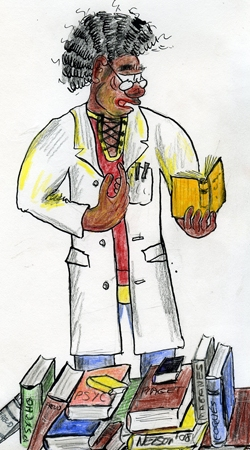
\includegraphics[height=60mm]{corps/chapitre11/img/personnage-robespierre-psy.jpg}
\end{floatingfigure}

Tandis que Robespierre, lunettes rondes sur le bout du nez et sarrau de clinicien par-dessus son chandail de football, est profondément plongé dans l’intimité de Marceline, cela depuis un gros dix minutes, Timothée, les yeux cernés comme il ne les a jamais eus, se sert de la fonction téléphonique du quanticordi pour essayer de se procurer un nouveau DPP. En même temps, les enceintes diffusent du Dylan :

    Combien de fois un homme doit-il regarder en l’air
    Avant de voir le ciel ?
    Oui, et combien d’oreilles doit avoir un seul homme
    Avant de pouvoir entendre pleurer les gens ?
    Oui, et combien faut-il de morts pour qu’il comprenne
    Que beaucoup trop de gens sont morts ?
    La réponse, mon ami, est soufflée dans le vent,
    La réponse est soufflée dans le vent.

Timothée lève les yeux.

- Dis, Robespierre, tu baisses ta musique, un peu ?

- Ça se peut-y que tu ne l’ait pas rechargé ? fait la voix du technicien. J’demande ça d’même …

- Non. Ç’a rien à voir, je l’ai toujours bien rechargée, ma fichue boucle d’oreille.

- T’es bien certain ?

- Oui !

- T’es certain que t’as pas pris ta douche avec ?

- J’suis pas si cave que ça ! Dites donc, vous me prenez pour qui ?

- Ouh ! Y est pointu à matin, le Motté !

- Oui, vous avez raison, je suis un peu fatigué.

- Grosse fin de semaine ?

- Ouin, c’est ça.

- OK. Rappelle-moi tes coordonnées.

- Timothée Tardif, CS-1, 5e Nord.

- OK. T’as rien qu’à passer avec ton vieux DPP, j’vas t’le changer.

- Parfait, à tout à l’heure !

Le premier message de sa boîte vocale est de Claude Sey, ce jeune agent de communication à l’emploi de Philippe «Flipper» Dauphin qui demande qu’on le rappelle le plus tôt possible en mode confidentiel. Ce que Timothée s’empresse de faire. C’est ainsi qu’il apprend que Louis-Marc Richard, son abject voisin de la rue Crouet, a reçu la visite d’un gorille du Flipper et qu’au terme, un rapport de six pages a été entré dans le système. Pire, une demande officielle d’enquête vient d’être acheminée au service de la sécurité. Ce serait en rapport avec le Dr Gagnon.

- À bon entendeur !

- Merci monsieur Sey.

Robespierre le fixe de ses grands yeux interrogateurs, ceux qui intimident habituellement Timothée.

- C’est quoi déjà le cliché habituel, Robespierre ? Ah oui : «l’étau se resserre».

- Qu’est-ce que tu veux dire ?

- Je viens d’apprendre que j’ai la Sécu aux fesses.

- T’as vraiment pas une vie singulière, toi. Je suis très heureux de te connaître.

- Merci.

- Mais là, j’ai un gros problème. Il faut que je relise bien attentivement et c’est pas facile. Y a tellement de fautes que c’est parfois illisible. Ensuite, va falloir que je réfléchisse. Va peut-être falloir que je bouquine pour bien comprendre. Donne-moi une couple d’heures. C’est trop délicat, je veux pas te donner n’importe quel conseil.

- Merci.

Le colosse lui fait signe de déguerpir.

Privé de Saguewanish, le CS-1 démarre sa tournée routinière du matin, à pied, une démarche surréaliste compte tenu de tout ce qui lui pend au bout du nez. Comment peut-on se promener à ne rien foutre dans un couloir qui empeste le vieux alors que tout foire autour de soi ? «Comment peut-on danser quand notre Terre tourne ? Comment peut-on dormir quand nos lits sont en feu ?» Comment peut-on respirer quand nos aînés sont nourris avec ce margouillis de Nutrisuz ? Comment peut-on ne pas fuir, là maintenant, pour l’île d’Anticosti ? Pourtant, le salon communautaire semble normal; le 500 y bat son plein avec ses accrocs habituels, les Marven, Beaulieu, Jean et compagnie. Mais assis dans le fond, à quelques mètres de Mme Bellow, le couple Martel est en conversation. Nouveau ça ! Y caresse-t-on des projets ? S’y remémore-t-on le passé ? Va-t-on demander une autre nuit d’intimité ? Un peu plus loin, devant l’écran du terminal quanticordi CLTD, Mme Labbé s’emmerde à regarder de vieux clips pas de son. Est-elle brouillée d’avec sa copine Thériault qui a d’autres chattes à fouetter ? Ici, la dame à moitié chauve essaie de ne pas somnoler devant la télé dont on a coupé le son, là Jean Saint-Gelais semble être à l’affut d’un mauvais coup à faire.

Comme il quitte pour cheminer jusqu’à la première salle 2P, Marie-Odile descend de l’ascenseur, en équilibre sur sa bécane. Apercevant le chef de section, elle le hèle à la manière d’un sergent-major à moustache et, l’accélérateur au maximum, fonce sur lui. Son visage aux antipodes de celui qui se béatifiait dans les langueurs lascives, charnelles et méritées du week-end, est devenu celui d’un inspecteur cocu qu’on a rétrogradé à la circulation et qui entend le faire payer très cher aux automobilistes, ces salopards. Le fils de la Maririou sait maintenant à quoi s’attendre. Froidement, sans dégainer, de toute façon les agents de la Sécu ne sont pas armés, elle lui ordonne non pas de s’appuyer les mains au mur et d’écarter les jambes, mais de la recevoir chez lui, dans son officine, à porte fermée, officiellement !

À peine assise, le verbe venimeux, l’œil pugnace et la griffe sortie, elle se dit d’abord «excessivement déçue». La direction générale lui a demandé, ce matin, d’enquêter sur le CS-1 Timothée Tardif. Mercredi dernier, dans la matinée, sur le temps du CRG, il aurait été vu en consultation précipitée à la clinique privée du docteur Étienne Gagnon, soi-disant pour une urgence. Tous deux seraient partis sur les chapeaux de roue, malgré les patients qui attendaient leur tour. Or il a été établi que le docteur Gagnon n’est pas passé au Centre ce jour-là. Question : si l’urgence ne concernait pas des bénéficiaires du Centre et si, lui, Timothée, semble ne pas avoir besoin de soins d’urgence, si c’est vrai ce qu’il dit à «ceux ou celles qu’il amène manger au Vieux Cormier» à savoir qu’il n’a pas de vie en dehors du Centre et de son domicile à Nazareth, à qui étaient destinés les soins d’urgence ? Et que penser de cette déclaration d’un certain Louis-Marc Richard, déclaration consignée par Philippe Dauphin devant témoin, selon laquelle il se passerait des «choses étranges» dans la résidence dudit Timothée Tardif ?

Si on fusionne ces deux rapports, n’est-on pas en droit de se poser de sérieuses questions ? Par exemple, qu’il pourrait y avoir des embrouilles probablement répréhensibles dont Timothée ne lui a pas parlé à elle qui s’était abandonnée à lui. «Après tout ce qui s’est passé», il aurait pu, au moins, avoir la décence de tout lui dire ! Mais pour cela, il aurait fallu qu’il lui fasse confiance. Qu’il s’intéresse à autre chose qu’à la bamboula. Bref, elle est blessée, elle se sent flouée, elle se croit trahie. Et elle, la femme flic, elle veut savoir ce qu’il en est. Maintenant ! Avant qu’elle n’aille interroger le docteur Gagnon et le dénommé Richard.

Un jour, Timothée avait peut-être dix ans, l’auto familiale s’était fait arrêter pour excès de vitesse. Furieux, le patrouilleur avait remis sa contravention à un Romain très silencieux, puis s’en était retourné dans sa voiture banalisée en faisant claquer la portière.

- Pourquoi il n’est pas content le monsieur ? Parce que quand il m’a intercepté la semaine dernière, il m’a donné une chance. Mais aujourd’hui, il voit bien que je n’ai rien compris. Il est déçu, il me laisse tomber et il me colle un sacrament de gros ticket !

Cette histoire lui était restée dans la tête et il regarde maintenant Marie-Odile avec la sensation que les carottes sont cuites. Un instant, il songe aux pilules du bonheur. En serait-on rendu là ? Comment serait-ce possible qu’on ne le soit pas, qu’il n’ait pas à poser un geste définitif en remettant les cachets à ses parents ?

Pour un ex-puceau de fraîche date, sa réponse est habile.

- Ça rien à voir avec toi en tant que femme, mais avec toi en tant que police. Je ne t’ai rien dit parce que si je le fais, tu vas devoir faire un rapport, ce qui déclenchera mon congédiement et bien pire encore. J’ai pas passé la fin de semaine avec une flic, mais avec une femme. Et j’ai aimé ça.

Elle encaisse le coup.

- Mais c’est quoi qui faut pas que je sache qui est si important ?

- J’peux pas te le dire. Notre conversation est probablement en train d’être numérisée par la microcam intégrée dans le premier bouton de ta chemise, ce gadget dont tu m’as parlé vendredi midi à la pizzeria, et c’est relayé au 2e étage comme pièce incriminante devant être versée à mon dossier. Désolé, ajoute-t-il en lui tendant les poignets, écris dans ton rapport que j’ai refusé de collaborer.

- Pour l’instant, personne ne m’a encore demandé d’enregistrer quoi que ce soit. Mais juste au cas …
Elle extirpe d’une de ses poches de bermuda un zinzin noir de la taille d’un cube de sucre. Du pouce, elle l’écrase : clic !

- Les ondes sont maintenant brouillées; c’est plus possible de rien numériser.

Il lui scrute longuement les yeux et ce qu’il y discerne l’incite à plonger, allez savoir pourquoi. Alors, il raconte tout. La coke, le feu, Alessandro, la loi du Gros Turcotte, le sous-sol, le voisin chiant, la maladie de sa mère, le docteur Gagnon, les conditions épouvantables de paiement et son désarroi. Il omet cependant de mentionner cette lettre qu’il a remise tout à l’heure à Robespierre. Pourquoi l’aurait-il fait ? N’y parle-t-on pas de meurtre au premier degré avec circonstances atténuantes discutables ? L’heure que nécessitera cette confession sera ponctuée de coups frappés à sa porte et de sonneries de téléphone : Ronnie Ross, de 8 à 4 cette semaine, qui veut lui parler du père Jean, Solange Gadoury qui insiste pour faire valoir un point de vue, l’infirmière Béatrice Martin qui offre son aide s’il le juge nécessaire et Shimoune Saint-Pierre qui affirme avoir de l’info intéressante pour lui.

- Ton histoire a tellement pas de bons sens qu’elle doit être vraie !

- Je t’ai tout raconté. Et maintenant ?

Elle se lève et se place les mains sur sa Saguewanish.

- Et maintenant, je vais réfléchir.

Comme elle ouvre la porte, Robespierre apparaît.

- Tiens, bonjour Marie-Odile, lui serine-t-il les lèvres tout en appétit.

Elle le salue sèchement de la tête, hésite un instant et file vers l’ascenseur. Elle a oublié de désembrouiller les ondes.

- Tu peux parler librement, le nécessaire a été fait pour que ça soit impossible de numériser les conversations.

- Méchantes belles relations !

- Et alors ?

- B’en ça m’en dit beaucoup sur toi et sur ta mère.

Et voilà le Robespierre, docteur Robespierre, en frais de décortiquer la longue lettre de Marceline et d’interpréter ce qu’il y a découvert comme états d’âme, nature humaine, traits de personnalité, séquelles psychologiques, voire dommages permanents, le tout à l’aide de ses maîtres à penser, certains étant cités dans le texte. Ainsi, Marceline n’est pas la dépendante affective typique qui a besoin d’être prise en charge, dominée, par un homme. Elle n’est qu’une malchanceuse qui s’amourache d’un beau voyou, Edmond Rioux, qui arrive à la battre simplement parce qu’il est beaucoup plus costaud qu’elle. Sinon, c’est probablement elle qui le rouerait de coups. Le gars est une brute qui idéalise la violence laquelle est confondue avec expression de la virilité et sens de la réplique. Ce que Marceline ne conteste pas, du reste. Les bagarres de son époux dans les bars, sa valorisation masculine, son obligation de la violer pour commettre l’acte sexuel, sa facilité à frapper sa fillette, sans oublier sa misogynie évidente, sont autant de pistes pour supposer que ce personnage est un homosexuel refoulé.

- Il y a soixante ans, personne ne quittait son placard. On se contentait de prouver le contraire en battant tout le monde. C’est simple : en 1962 «tapette» égalait «fif qu’on roue de coups» et «vrai gars» égalait «brute virile hétéro que l’on craint». Ce que je dis est tellement documenté que c’est quasiment devenu un poncif.

Quant à Marie, ses réactions sont toutes conformes au manuel, soutient le psychologue autoproclamé. Élevée sans tendresse, elle grandit dans la crainte d’un homme immense, bruyant, imprévisible, alcoolique, violent et dangereux, bref, un ogre épouvantable. Elle s’habitue à une mère disgracieuse, une femme violée, violentée, incapable de se faire respecter et de protéger son enfant, une malheureuse qui tente d’oublier en jardinant, en buvant et en s’acoquinant au village pour au moins avoir quelqu’un à qui parler, autrement dit, une personne en grand désarroi, en grande souffrance. La petite fille est amenée à la musique, à la culture et au savoir, elle est initiée à la tendresse, à la générosité, au respect et à la valorisation, par son institutrice, la seule à voir en elle autre chose qu’une misérable Bezo sur qui on peut taper sans conséquence.

- En gros, il y a une sorte d’image manichéenne qui s’est formée dans son esprit de survivante : d’un côté le monde des méchants, de l’autre celui des gentils. Dans le premier, il n’y a pas de musique, dans l’autre, il y en a. J’ignore ce qu’il en est dans sa vie, à ta mère, je n’ai jamais eu le plaisir de la rencontrer, mais, à la lecture du document, je ne serais pas étonné d’apprendre qu’elle ait passé sa vie à trembler devant les forts en gueule, les gros bras, les meneurs de claques, les clous de soirées ou encore les hommes qui semblent s’intéresser à elle sans qu’elle ne l’ait décidé. Je suppose que ton père, pour qu’il soit ton père et qu’elle tolère qu’il continue de l’être, a dû être tout le contraire, toute sa vie, c’est-à-dire un homme doux, tolérant, facile à vivre, de bonnes compagnies, qui lui a toujours passé ses caprices et ses volontés. Ai-je tort ?

- T’es dedans à 100 %.

- J’en déduis qu’elle t’a élevé pour que tu ne sois pas un mâle alpha, pour que tu sois vraiment doux, presque silencieux, sobre, fidèle, solitaire comme elle et dévoué à sa personne, voire capable d’en prendre soin sur ses vieux jours. Mais ça, je n’ai pas à te demander ton avis, je sais que tu as ce genre de comportement.

Un comportement n’ayant que fort peu à voir avec celui du vrai Timothée de Milet, l’homme de la Lyre à onze cordes.
Un frappement précède l’ouverture de la porte. Ronnie Ross se fait insistant.

- Excuse, Motté, siffle-t-il en ignorant Robespierre, ce qui est la chose habituelle à faire, mais faut que j’te dise au sujet du pére Jean. Ils l’ont descendu au sous-sol.

- Qui ça ? La Sécu ?

- Ouin. Tropecolo le Chinois et Tremblay la Bitch. Paraîtrait que c’est lui qui a bousillé ta saguigui.

Timothée réfléchit un instant.

- C’est quoi le topo avec les bénévoles cette semaine ? Depuis vendredi, le père Jean passait ses fins de journée avec monsieur Lafrance en 3P-L. Si c’est comme la semaine dernière, on a un problème.

- Ouin, le bonhomme ‘i est rendu écœurant; faut ‘i changer ses couches aux heures. J’en n’ai jamais vu des puantes de même ! On n’a rien qu’à le transférer en palliatif, la cérémonie va avoir lieu dans une semaine. D’ici c’temps-là, on va pouvoir s’arranger.

- J’vais y penser. En attendant, peux-tu vérifier pour les bénévoles ?

- J’vas aller voir.

Le préposé parti, Robespierre s’assure que la porte est bien refermée et il poursuit ses explications.

- Comme résultat de son enfance, ta mère a probablement peur de s’impliquer avec les gens, de travailler en équipe. Elle va rechercher la solitude, fuir les mondanités, la société. Par instinct, par méfiance, par réflexe de survie, elle refusera de s’ouvrir, d’échanger de façon intime. Elle craindra qu’on lui fasse mal. Elle voudra se protéger. Et si ça se peut ce que je viens de dire, sa vie sexuelle sera misérable. Pour elle, faire l’amour équivaudra à se laisser aller avec un homme désireux de la posséder, la soumettre, la violenter. Dès lors, l’image impitoyable, brutale, douloureuse du père se substituera. Mais ça, il est plus que probable que tu ne le saches pas; par contre, ton père, lui …
Timothée hoche horizontalement de la tête. Va pour la vie sexuelle, mais pour s’impliquer avec les gens, c’est une autre histoire.

- Toute sa vie, elle a été musicienne, elle a joué dans des orchestres symphoniques importants, ici, elle s’est occupée de l’École de musique…

- Ce n’est pas parce que tu joues dans un orchestre symphonique que tu es attentif aux autres; tu es peut-être claquemuré dans ton monde à toi en train de lire des partitions, parce que la musique est la seule thérapie qui t’ai gardé en vie. Mais écoute, Timothée, mon échafaudage n’est que de la théorie; je ne connais pas ta mère du tout. Et puis je suis loin d’être un psy; je ne suis que Robespierre Alcide, arrière-petit-fils de l’inventeur du Pétépano. Quant à ta question de ce matin sur le document, à mon avis, il faut le donner à ta mère en lui disant toute la vérité. Ça lui revient. Béatrice Martin te l’a remis, toi et ton père vous l’avez lu parce que vous n’aviez aucune idée de quoi il s’agissait. Maintenant que vous le savez, vous croyez vraiment que ça peut lui faire du bien de le lire, pour peu que son contenu soit vrai, et, surtout, vous n’en dites pas plus, vous ne lui laissez pas sentir que vous aimeriez en parler.
De nouveaux coups se font entendre. C’est encore Ross, mais cette fois il se bouscule littéralement avec la mère Gadoury et il finit quand même par entrer.

- Méchant problème, Motté. Ils nous ont pas trouvé de bénévoles cette semaine. Va falloir se débrouiller.

- Y est pas question que vous transfériez Lafrance au mouroir, griche Mme Gadoury, ses petits doigts boudinés faisant comme s’ils étaient griffus.

Le CS-1 enlève ses verres pour se frotter les yeux et il fixe Robespierre en haussant les épaules. Le colosse se lève aussitôt et disparaît dans le large couloir.

- Toé, le vieux hibou, tu te mêles pas de nos affaires, t’as-tu compris ?

- Ronnie, câlisse ! Mme Gadoury veut juste … Ah bof !

Un instant, plus personne ne parle.

- Bon. On va se démerder comme le mois dernier; on va mobiliser nos bénéficiaires des salles 2P. Tant pis pour les humeurs !

Sentant qu’il pourrait lui en cuire - n’est-elle pas elle-même hébergée en salle 2P ? – Solange Gadoury disparaît dans le sillage de Robespierre Alcide.

Arrivés au poste de garde, Timothée, Ronnie et Steve Grenier, l’autre préposé assigné cette semaine au 8 à 4, ont tôt fait, liste en main, d’affecter leur clientèle la moins «poquée» selon les besoins du premier et du deuxième quart de travail. Tout le monde y passe, incluant Mmes Gadoury et Bellow. La première pour faire une fleur à Ronnie, la seconde parce que le CS-1 entend la ménager à sa façon.

- Madame Bellow, suivez-moi, lui dit-il, une demi-heure plus tard quand tout un chacun, dans un concert d’indignations, a reçu son affectation.

Docile, la vieille dame lui emboîte le pas.

- Je vous vois mal passer la moppe, donner le manger mou aux impotents ou changer des couches en salle palliative.

- Mais si, je peux faire ma part.

- Je le sais, mais il y a mieux à faire. Vous connaissez monsieur Alcide ? lui demande-t-il en cognant à la porte de Robespierre.

- C’est pas barré, entend-on.

- Mon ami monsieur Alcide, voici madame Bellow, détentrice d’une maîtrise en bibliothéconomie de l’Université de Montréal.

Le sportif réglementé reçoit cette preuve d’amitié comme un pavé d’asphalte tombé dans sa soupe.

- Avez-vous déjà vu ça, madame Bellow, un bordel de livres comme ça ?

- Non, monsieur Tardif.

Robespierre n’ose parler.

- Écoute, madame Bellow est bénévole pour te conseiller dans ton classement. Entre diplômés universitaires et rats de bibliothèque, vous allez sûrement vous entendre.

- C’est très gentil, mais … je me comprends très bien dans mon bordel !

- Regarde, c’est rien de vraiment compliqué. Il s’agit seulement de t’assurer que Ronnie ou Steve ne l’attraperont pas pour l’envoyer changer les couches de monsieur Lafrance ou laver les toilettes dans les 3P. Défends-la sur ton honneur de grand chevalier noir. Et, qui sait, peut-être qu’en retour, elle va vraiment t’aider dans ton foutoir.

Et là-dessus, le CS-1 file vers l’ascenseur. S’il a de la chance, il pourra descendre au soutien technique, situé au rez-de-chaussée sud, où on lui remettra une nouvelle boucle d’oreille. Mais il n’en a pas; c’est comme si la fatalité s’acharnait à le priver de moyens de communication et de transport. Cette fois, c’est Marie-Odile qui l’attend au poste de garde. Elle a quelques papelards électroniques à lui faire signer relativement au sabotage de sa Saguewanish. Au moment où elle lui tend le stylet, Steve Grenier, une des pires langues du CRG-BSL passe et les gratifie d’un sourire narquois.

- T’as d’la belle visite, le Motté ?

La femme flic lui lance un regard tellement mauvais que le grossier personnage entreprend de se fondre dans le revêtement mural. Replaçant le mini ordi tactile dans sa petite housse en cuir, elle lui raconte que durant la fin de semaine, son collègue David Gagnon- Tropecolo, alias Tropecolo le Chinois pour cause d’épousailles avec une dame de Shanghai, a ouvert une enquête et s’est promené sérieusement dans les locaux du 5e Nord. Il n’a pas mis trop de temps à repérer quelques maillons faibles dans la défense du suspect et à les faire craquer un à un. Trois témoins ont signé leur déposition inculpant Jean de méfait sur des biens de la couronne. Redoutable le Tropecolo !

- Ce matin, en arrivant, il est parti se chercher une autorisation chez Carl Michaud. Ça nous a permis, lui et moi, d’aller ramasser le bonhomme ici à côté dans le salon et de le descendre en bas dans un «local de réflexion».

- Vous allez faire quoi avec ?

- Rien. Il va croupir là au moins jusqu’à l’hiver. La direction générale a décidé de pas porter plainte à la police.

- Ça va se régler à l’interne.

- C’est ça.

Est-ce dû à la gêne qui s’ensuit ? C’est comme si, de cette crevasse de silence qui s’est excavée entre eux, on préférait subir le dégagement des gaz volcaniques, le grondement des entrailles de la Terre et le surgissement des démons de l’enfer. C’est Marie-Odile qui casse néanmoins la glace.

- J’achève ma réflexion et j’aimerais t’en faire part.

- Bien sûr. Euh … Tropecolo est-il au courant pour mon histoire avec le docteur Gagnon ?

- Non. C’est mon dossier.

La bonne nouvelle, elle est seule sur l’affaire. La mauvaise ? Elle est seule sur l’affaire !

- Tu pourrais passer chez moi, ce soir vers 19 heures, si ça te convient.

- Ça marche. Mets une bouteille au frais, ajoute-t-il en le regrettant instantanément.

Pourquoi a-t-il dit cela ? Qu’est-ce qu’il lui a pris ! «Quel idiot tu peux être», le chicanerait sûrement Quetzalcoatl. Marie-Odile ne semble pas l’avoir apprécié non plus, car elle vient de repartir en le gratifiant ni d’un sourire, ni d’une formule polie. Samedi soir, elle lui avait pourtant prouvé qu’elle pouvait avoir de si jolis yeux.

- Motté, lui crie Ronnie Ross.

- Quoi ?

- Y a le gros Lavoie en ligne. Il veut savoir si tu as vu la mère Morency.

- Non je n’ai pas vu madame Morency.

Luce Morency, le lac Saint-Mathieu, les roulottes. Sa mère farouchement seule avec sa musique. Son père qui venait les retrouver le soir après sa journée de livraisons. À cette époque, faisaient-ils encore l’amour ? Pourquoi aujourd’hui n’en a-t-il pas de vagues souvenirs d’enfance, ceux d’une porte mal fermée, d’une preuve de tendresse, de soupirs à peine étouffés, d’un geste inconvenant, d’une complicité amoureuse ? Et si Robespierre Alcide avait raison ? Si la Maririou était sexuellement handicapée ? Le degré d’improbabilité de sa naissance à lui, Timothée, serait beaucoup plus élevé qu’il ne le croyait. Et, tant qu’à pousser dans la réflexion inavouable, Romain le Gelé était-il homme à se priver de vie sexuelle en raison d’une conjointe foquée ? Probablement pas. Auquel cas, avait-il des maîtresses ? Comment le savoir ? Et pourquoi, au juste, faudrait-il le savoir ? À qui cela profiterait-il ?

Arrivé au rez-de-chaussée, le CS-1 veut gagner les locaux des services techniques, tout au fond. Mais Shimoune Saint-Pierre lui fait signe. C’est vrai, il allait l’oublier celui-là. Timothée se dirige donc vers la cafétéria sauf que, au sortir du grand escalier menant au sous-sol, Gagnon-Tropecolo dit le Chinois fait son apparition.

- Ah, monsieur Tardif, lui lance-t-il, vous tombez bien.

\begin{floatingfigure}[l]{40mm}
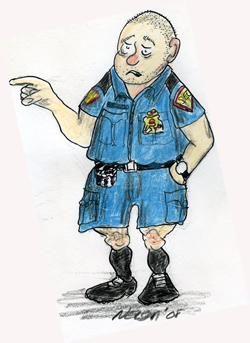
\includegraphics[height=60mm]{corps/chapitre11/img/personnage-tropecolo.jpg}
\end{floatingfigure}

Il arrive du «centre de réflexion» pour cette histoire de Saguewanish sabotée où, raconte-t-il, il a hérité d’un problème. Depuis la semaine dernière, on y héberge, sans trop de motifs apparents, un certain Robert Gagnon, pas parent avec lui soit dit en passant; lui, sa mère est une Gagnon du Témiscouata qui a épousé Gian-Maria Tropecolo, un montréalais de la Piccola Italia. Toujours est-il qu’il y a embrouille. Le dossier du monsieur semble être chez Philippe Dauphin, le directeur des communications, une procédure tout à fait inhabituelle. Or, ce Gagnon, mieux connu ici et là sous le nom épouvantable de Dart Vader, relève du 5e Nord.

- Y a rien à comprendre là-dedans.

- Faut demander à Dauphin.

- Je peux pas, il est parti jusqu’à demain.

- Qu’est-ce que vous voulez que j’y fasse ? Il m’a passé carrément par-dessus la tête, Dauphin. Il a fait incarcérer mon bénéficiaire simplement parce qu’il avait un petit peu chialé à la télé contre le Centre.

- Si personne n’est là pour justifier l’incarcération, on ne peut garder le monsieur. Il doit sortir. Comme vous êtes son CS-1, prenez sur vous pour le faire sortir.

- Je peux ?

- Ben oui, vous signez la levée d’écrou, c’est tout. On n’est pas encore retourné au temps de Louis XIV et des lettres de cachet.

Intéressant le Chinois. Pour un flic !

Une minute plus tard, l’agent se retrouve avec Timothée devant une porte de cellule en compagnie de deux armoires à glace, les frères «Papynut» et «Bluesly» Côté. Sur chaque porte de cellule, un écran HD tient lieu de fenêtre. En l’occurrence, on voit Dart Vader, écrasé sur un petit lit, en train de regarder un téléviseur fixé au mur. Tropecolo tapote l’écran et, pouf !, l’image vidéo cède la place au dossier du bénéficiaire.

- Vous voyez ici, explique-t-il au CS-1, aucun motif n’apparaît au dossier pour son incarcération. Et si vous questionnez les PapyBlues – il pointe vers les deux affreux - vous allez apprendre qu’on l’a installé ici sans avoir complété la paperasse habituelle.

- Nous autres, les boss nous ont dit d’ouvrir une cage pour mettre le bonhomme. Fait que, on l’a faite, ’stie ! Clac !

- Ça n’a pas de bon sens !

- C’est ce que je pense. On le relâche ?

- Ça va de soi, répond Timothée.

Tropecolo fait signe à Papynut, à moins que ce ne soit à Bluesly, lequel, qui qu’il soit, commande l’ouverture de la porte de son DPP. Une senteur fauve de vieillard en panne d’hygiène agresse alors les quatre employés. Effectivement, Dart Vader ne s’est pas lavé depuis mercredi dernier, ce qui ne semble pas l’embarrasser. Il s’assoit sur son grabat et appuie sur sa canule.

- Tiens, si c’est pas le chef ! Flipper a eu peur de venir lui-même ?

- Vous pouvez retourner au 5e, monsieur Gagnon, lui répond Timothée. On s’en parlera.

Tandis que le bonhomme déguerpit sans demander son reste, le CS-1 autorise la «libération» directement sur le moniteur de la porte. Taptap ding ! Il est à prévoir que Dauphin ne sera pas particulièrement heureux de l’initiative. Mais on ne peut quand même pas priver un vieillard du peu de qualité de vie qui lui reste par crainte de froisser un ego. De toute façon au point où il en est, le fils de la Maririou s’en fiche.

Les deux gardiens qui en ont vu bien d’autres, saluent leurs visiteurs et s’en retournent dans leur antre, «probablement pour y croquer de petits enfants» songe Timothée. Au même moment, une voix connue se fait entendre derrière lui.

- On se dirait dans un pays barbare.

Il reconnaît le docteur Bellavance.

- Sinistre, le sous-sol, non ? Des entrepôts de produits chimiques, des geôles, des prisonniers hagards, sales, édentés, des janissaires monstrueux, un savant fou ! Comme dans les pires dictatures ! Comment allez-vous, monsieur Tardif ?

- Euh, ça va, merci. Et vous docteur ?

- Vous ne voulez pas le savoir, monsieur Tardif, vous ne voulez pas le savoir.

- Euh …

- Un jour, vous viendrez visiter ma petite installation, juste là-bas, les grandes portes blanches. On parlera.

- Au revoir, docteur.

- Au revoir Monsieur Tardif.

En refaisant surface au rez-de-chaussée, Timothée décide de foncer, tête baissée, en direction des services techniques. Ainsi, il pourra se reconnecter aux systèmes informatisés de l’établissement. Quand on est habitué à avoir accès à tout, aux locaux, à la géolocalisation, à la téléphonie, à la messagerie, à ses horaires, à son agenda, à son aide-mémoire, à un magnétophone, etc., directement d’un gadget gros comme un bleuet, un DPP, on se retrouve lourdement handicapé lorsqu’on en est privé. Pour le moins ! Mais comme il a peine à se contenir la vessie, il bifurque par les latrines du secteur. Mal lui en prend. Au moment où, sa vidange complétée, il est en train de se laver les mains, il aperçoit dans la rangée des cubicules d’aisance que lui reflète le miroir, deux pieds nus tout recroquevillés, des pauvres pieds raccordés à de misérables jambes rougies et atrophiées par le temps.

Sans hésiter, il cogne à la porte du petit compartiment.

- Il n’y a personne, chantonne la voix de Luce Morency. C’est une erreur.

- C’est vous madame Morency ?

- Je me suis trompée de salle.

Pendant plusieurs minutes, le CS-1 essaie de convaincre la démente de lui ouvrir. Et lorsqu’il y parvient, il la trouve assise, aussi nue et perdue que lors de ses autres fugues.

- Venez, madame Morency, on va s’en aller.

- Mais il faut que j’aille aux toilettes; ici, c’est pour les hommes, je me suis trompée.

- Je comprends. Venez, je vais vous montrer le chemin.

Il l’entraîne par la main et lui ouvre la porte marquée du symbole féminin.

- Prenez bien votre temps, madame Morency, je reviens tout de suite.

Timothée entend faire d’une pierre deux coups. Il va aller aux services techniques prendre livraison de sa nouvelle boucle d’oreille et il va lancer un code magenta à l’attention du sixième. Mais sur place, manque de chance, un petit écriteau avertit que le personnel ne sera de retour qu’à 13 h 30.

- C’est pas vrai !

Miraculeusement, une préposée poussant un chariot de prélèvements et de pots d’urine, cling cling cling, vient le tirer d’affaire. Il lui fait lancer l’appel d’urgence avec son DPP et il lui demande de bloquer l’accès aux toilettes le temps qu’on descende chercher la vieille dame. Celle-ci est assise en boule le long du mur, entre les lavabos et l’essuie-mains, toute grelottante en raison de l’air climatisé. Timothée s’accroupit à côté d’elle.

- Je vous connais …

- Oui madame Morency. C’était dans le temps, au Lac-Saint-Mathieu. Vous rappelez-vous ? Vous aviez un commerce de vieilles maisons mobiles et l’École de musique vous en louait quelques-unes chaque été. En tout cas, pendant quelques étés d’affilée, quand j’étais petit, madame Morency. Celle que ma mère occupait, une roulotte tout croche et en retrait des autres à cause d’un tas de roches, immense, merveilleux, plein d’embûches – j’en avais fait mon terrain de jeu - lui servait surtout à donner des leçons aux quelques étudiants qui avaient remporté un séjour au lac.

- Le lac …

- Les soirs, parfois, mon père venait nous trouver. On allait prendre une marche jusqu’à la bergerie. Les moutons venaient me voir. Je pouvais les flatter. Ils avaient de drôles d’yeux, les moutons. Ça me faisait bien rire. Ma mère elle, elle restait à la roulotte pour pratiquer son violoncelle. Ç’a été l’histoire de sa vie, la musique. Il n’y a jamais eu de vraie place pour rien d’autre …

- Vous connaissez le lac …

La porte s’ouvre brusquement et le gros Lavoie apparaît armé d’une couverture.

- Coudon, le Motté, on dirait qu’a te courre après, la bonne femme.

- Étouffe-toi donc, gros sans dessein !

Aussitôt articulée, l’invective l’étonne encore plus que Lavoie qui n’en croit pas ses oreilles. Pour la première fois de sa vie, Timothée vient de rabrouer quelqu’un. Et pas n’importe qui, le gros Lavoie, un des pires malfrats du Centre, le copain du redoutable Pierre Monger. Il se doute bien qu’il y aura représailles, mais pour l’instant, il méprise les ricanements sournois qu’il entend et repart en direction de son 5e Nord. Comme il sort de l’ascenseur, il croise Steeve Desrosiers, son collègue CS-1 du 5e Centre chevauchant une rutilante Saguewanish flambant neuve.

- As-tu oublié la réunion ?

Timothée hausse les épaules.

- Quelle réunion ?

- La TCS.

- Et merde ! Je me dépêche.

Une fois par mois pendant une demi-journée, les chefs de section du CRG-BSL se réunissaient en un comité officiel appelé Table des chefs de section (TCS), une perte de temps d’un ennui mortel conçue, initialement, pour faire le point sur leur situation. Sauf que c’était devenu une occasion d’étaler sa supériorité, de vanter ses prouesses gestionnaires et de raconter les pires anecdotes sur les bénéficiaires. C’est de cette façon que Timothée engloutira son après-midi. Il n’aura ni le temps d’aller parler avec Dart Vader, ni d’aller rencontrer Shimoune Saint-Pierre, ni de s’occuper de sa boucle d’oreille, ni de prendre des nouvelles de sa vieille saguigui, ni de s’informer sur la viabilité de l’association Bellow – Robespierre. Par contre, en arrivant chez lui en taxi vers les 17 h, il retrouvera sa mère apparemment tirée d’affaire, fraîche et dispose.

- Marie, ton maudit chien, j’suis p’us capable !

Romain tente de frapper le chien-rat du pied, mais l’animal esquive et gronde de plus belle.

- Y est pas normal c’te chien !

- Gajou, rechte à côté de Maman, chinon, tu vas payer pour.

- J’vas aller chercher des œufs dans le poulailler.

Romain ouvre la porte de secours et gagne la petite terrasse. La brise vient chasser quelque peu la fétidité de l’air intérieur. Timothée en profite, suivi de Gazou.

- J’ai parlé à Robespierre, dit-il au travers des caquètements et des aboiements du cabot.

- Pis ?

- Il faut lui donner la lettre. Il faut lui dire toute la vérité : qui nous l’a remise, qu’est-ce qu’on a fait avec. On sait pas si le contenu est vrai, mais on pense que ça va l’intéresser. Après ça, on n’en parle plus. On la laisse faire.

- Ça marche.

- Mais c’est pas tout. Louis-Marc Richard a commencé à parler et au Centre, ils se doutent de quelque chose.

- Ça veut dire quoi ?

- Ça veut dire que je sais pas quel bord ça va prendre. Mais juste au cas où ça foirerait, garde ça avec toi.
Il lui a remis la petite bouteille de pilules.

- Y en a deux.

Sans dire un mot, sans que rien ne paraisse dans son expression, Romain enfouit le contenant dans sa poche et gagne l’intérieur où il place ses œufs sur le comptoir.

Les yeux vers le fleuve, Timothée a peine à contenir ses larmes. Il voit bien que la conclusion approche, qu’il n’est plus possible de continuer, que le «Flipper» est en train de lui faire la peau, que Richard va continuer son œuvre de délation, cette fois auprès du BAG, que le docteur Gagnon va vouloir ses médicaments et qu’il ne pourra les lui donner, que Marie-Odile va venir mettre son nez dans leurs histoires, que ses parents vont peut-être devoir avaler les petits cachets de Robespierre, sans compter le reste. Et merde !

- On devrait laisser l’air entrer, il fait tellement beau, se contente-t-il de dire.

- Tu veux qu’on ch’fasse attraper ? Ils vont nous j’entendre de la rue !

Le fils referme la porte.

- Maman, dit-il, j’ai une lettre pour toi, une lettre qui remonte 66 ans en arrière et qui vient de ta mère. T’en fais ce que tu veux, mais Papa et moi on pense que tu devrais la lire.

La Maririou regarde l’épais document et n’ose lui toucher. Timothée le dépose alors sur la petite table à côté d’elle.

- Où ch’est que t’as eu cha ?

Il lui parle alors de Béatrice Martin, une petite-fille de Rose Joncas qui était l’amie de Marceline Belzile.

- Je la veux pas, ch’maudite lettre-là. J’l’ai pas voulue dans le temps, j’la veux pas plus à ch’t heure. Qu’est-che qu’elle avait à garder cha toute cha vie, ch’te vieille-là ?

Romain ramasse le document et s’approche du rayonnage mural.

- R’garde b’en Marie, je vais la mettre ici, ta lettre. Si t’as envie de la lire, tu la lis. Timothée me l’a lue, on voulait savoir si ça pouvait te faire du mal avant de te la remettre. Là, maintenant là, je pense que tu devrais la lire. T’as eu beaucoup de peine dans ta vie, mais c’te lettre-là, si ce qu’elle raconte est vrai, ça peut te faire du bien, te donner un peu de paix. D’un autre côté, si, dans ton coeur, tu es vraiment convaincue que la lettre est de la bouleshit, tu pourras te dire que t’as eu raison de penser de même pendant toutes ces années et, ça aussi, pourra te donner un peu de paix. Me semble, en tout cas. C’est juste toi qui peut le savoir. Cela dit, je t’en parlerai plus.

En guise de réponse, elle s’empare de son violoncelle, ce qui est le signal du cérémonial. Gazou file se cacher sous un lit, Romain va quérir son trombone et Timothée, convaincu que c’est possiblement la dernière fois qu’il vivra ce rituel, en fait autant avec sa fichue de clarinette, le cœur bien gros.

- Trio pour clarinette, violonchelle et piano, opuch 2 de Vinchent d’Indy.

Une bande d’enfants déboule en trombe sur la rue Crouet. Presque debout sur leurs vélos, ils passent sans les remarquer, devant Louis-Marc Richard qui, devant sa maison, est en discussion avec deux visiteurs qui semblent s’intéresser au faux cottage obstruant la vue du côté nord de la rue. 